% Created 2022-10-09 Sun 14:36
% Intended LaTeX compiler: xelatex
\documentclass[8pt]{article}
  \usepackage[letterpaper, portrait, margin=1in]{geometry}
  \usepackage[utf8]{inputenc}
  \usepackage[T1]{fontenc}
  \usepackage{amsmath}
  \usepackage{amssymb}
  \usepackage{hyperref}
  \hypersetup{colorlinks=true}
  \usepackage{tcolorbox}
% http://tug.ctan.org/macros/latex/contrib/minted/minted.pdf
  \usepackage[cache=false]{minted}
  \setminted{breaklines=true, breakanywhere=true}
% \usemintedstyle{paraiso-light} % pygmentize -L styles
% \usemintedstyle{emacs} % pygmentize -L styles
% \usemintedstyle{colorful} % pygmentize -L styles
% \usemintedstyle{rainbow_dash} % pygmentize -L styles
  \usemintedstyle{tango} % pygmentize -L styles
% https://tex.stackexchange.com/questions/112559/box-around-minted-environment
% https://ctan.math.utah.edu/ctan/tex-archive/macros/latex/contrib/tcolorbox/tcolorbox.pdf
  \BeforeBeginEnvironment{minted}{\begin{tcolorbox}[colframe=black!85!white, colback=black!5!white, boxrule=0.3mm]}
  \AfterEndEnvironment{minted}{\end{tcolorbox}}
  \usepackage{enumitem}
  \setitemize{itemsep=0.5pt}
  \usepackage{fancyhdr}
  \pagestyle{fancy}
  \fancyhf{}
  \usepackage{titling} % allows 	hetitle 	heauthor 	hedate
  \usepackage{lastpage}
  \rhead{\theauthor}
  \lhead{\thetitle}
% Disable pageref being a link https://tex.stackexchange.com/a/4599
  \rfoot{\thepage{} of \pageref*{LastPage}}
  \linespread{1}
  \setlength{\parindent}{0pt}
  \setlength{\parskip}{0.5em plus 0.1em minus 0.2em}
  \hypersetup{pdfborder=0 0 0}
  \setcounter{secnumdepth}{0}
%  \usepackage{fontspec}
%  \setmainfont[]{IBM Plex Sans}
%  \setmonofont[]{Iosevka SS14}

\usepackage{graphicx}
\usepackage{longtable}
\usepackage{wrapfig}
\usepackage{rotating}
\usepackage[normalem]{ulem}
\usepackage{amsmath}
\usepackage{amssymb}
\usepackage{capt-of}
\usepackage{hyperref}
\usepackage{fontspec}
\setmainfont[]{IBM Plex Sans}
\setmonofont[]{Iosevka SS14}
\author{Jonathan Fung}
\date{09/27/22}
\title{Artists in the USA}
\hypersetup{
 pdfauthor={Jonathan Fung},
 pdftitle={Artists in the USA},
 pdfkeywords={},
 pdfsubject={},
 pdfcreator={Emacs 29.0.50 (Org mode 9.5.4)},
 pdflang={English}}
\begin{document}

\maketitle
\tableofcontents

\begin{latex}
\pagebreak
\end{latex}
\section{Import}
\label{sec:org3e9438a}
Source: \href{https://github.com/rfordatascience/tidytuesday/tree/master/data/2022/2022-09-27}{tidytuesday - September 27, 2022}

\begin{minted}[]{r}
library(tidyverse)
library(mice)

tuesdata <- tidytuesdayR::tt_load('2022-09-27')
artists <- tuesdata$artists
options(crayon.enabled = FALSE)
\end{minted}

\begin{minted}[]{r}
head(artists)
\end{minted}

\begin{verbatim}
# A tibble: 6 × 7
  state      race   type  all_workers_n artists_n artists_share location_quotie…
  <chr>      <chr>  <chr>         <dbl>     <dbl>         <dbl>            <dbl>
1 Alabama    Hispa… Arch…         88165        45      0.000510            0.875
2 Alaska     Hispa… Arch…         26875        15      0.000558            0.957
3 Arizona    Hispa… Arch…       1033370       270      0.000261            0.448
4 Arkansas   Hispa… Arch…        101405        NA     NA                  NA
5 California Hispa… Arch…       7470730      3870      0.000518            0.888
6 Colorado   Hispa… Arch…        594525       200      0.000336            0.577
\end{verbatim}

\begin{latex}
\pagebreak
\end{latex}
\subsection{Impute}
\label{sec:org372c113}
We can inspect the data's missing values. There are 1909 complete records, and 1471 (17 + 755 + 699) incomplete records, rows that contain an NA value.

\begin{minted}[]{r}
md.pattern(artists, rotate.names = TRUE)
\end{minted}

\begin{center}
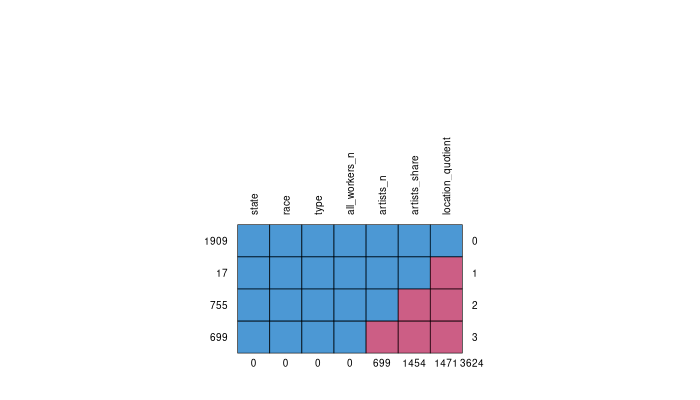
\includegraphics[width=.9\linewidth]{media/mdpattern.png}
\end{center}

Since this dataset has a high amount of missing data, we use Multiple Imputation by Chained Equations (MICE).

\begin{minted}[]{r}
imp_base <- mice(artists, m = 5, maxit = 0, print = FALSE)
mypred <- imp_base$pred
mypred[c("state", "race", "type"),] <- 0 # constants
## Sect 9: https://www.gerkovink.com/miceVignettes/Passive_Post_processing/Passive_imputation_post_processing.html
mypred[c("location_quotient", "artists_n"),"artists_share"] <- 0 # linear combination
mymeth <- imp_base$meth
mymeth["artists_share"] <- "~I(artists_n/all_workers_n)"

imp <- mice(artists, pred = mypred, meth = mymeth, maxit = 35, print = F, seed = 123)
artists_mi <- imp %>% complete() %>% as_tibble()
head(artists_mi)
\end{minted}

\begin{verbatim}
Warning message:
Number of logged events: 3
# A tibble: 6 × 7
  state      race   type  all_workers_n artists_n artists_share location_quotie…
  <chr>      <chr>  <chr>         <dbl>     <dbl>         <dbl>            <dbl>
1 Alabama    Hispa… Arch…         88165        45      0.000510            0.875
2 Alaska     Hispa… Arch…         26875        15      0.000558            0.957
3 Arizona    Hispa… Arch…       1033370       270      0.000261            0.448
4 Arkansas   Hispa… Arch…        101405        45      0.000444            0.962
5 California Hispa… Arch…       7470730      3870      0.000518            0.888
6 Colorado   Hispa… Arch…        594525       200      0.000336            0.577
\end{verbatim}
\begin{latex}
\pagebreak
\end{latex}
\subsubsection{Diagnostics}
\label{sec:orgbf70547}
We can check the general convergence of the MICE algorithm. Each row represents a variable that had missing data, with the LHS being the mean, and RHS being the standard deviation. A sufficient diagnostic plot should have no trends across iterations, which these mostly do.

\begin{minted}[]{r}
plot(imp)
\end{minted}

\begin{center}
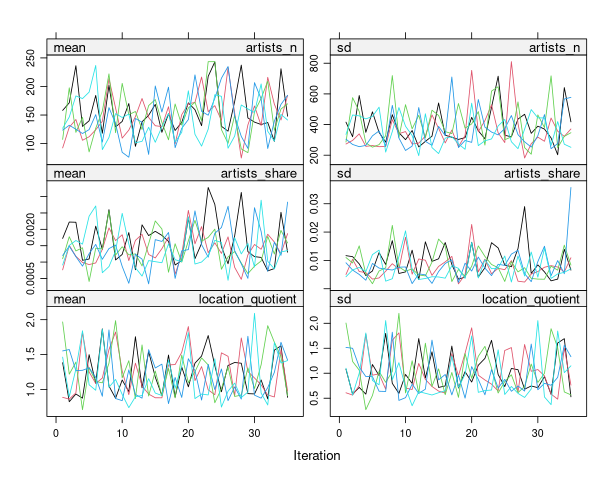
\includegraphics[width=.9\linewidth]{media/diag.png}
\end{center}


Next, we can show that the imputed values (Red) are within range (\emph{plausible}) of the original values (Blue):
\begin{minted}[]{r}
## https://stackoverflow.com/questions/2540129/lattice-multiple-plots-in-one-window
sp1 <- stripplot(imp, artists_n~.imp, scales=list(y = list(log = 10)), xlab = "", factor = 2)
sp2 <- stripplot(imp, artists_share~.imp, scales=list(y = list(log = 10)), xlab = "", factor = 2)
sp3 <- stripplot(imp, location_quotient~.imp, scales=list(y = list(log = 10)), factor = 2)

#library(gridExtra)
gridExtra::grid.arrange(sp1, sp2, sp3)
\end{minted}

\begin{center}
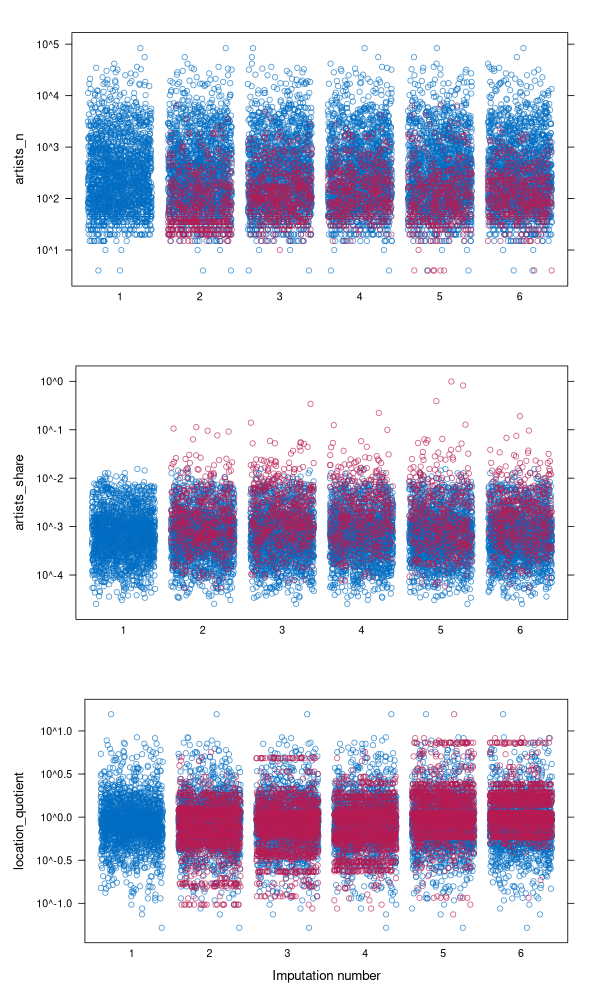
\includegraphics[width=.9\linewidth]{media/diag_range.png}
\end{center}

Similarly, we can inspect their distribution:
\begin{minted}[]{r}
densityplot(imp, scales=list(x = list(log = 10)), layout = c(3,1))
\end{minted}

\begin{center}
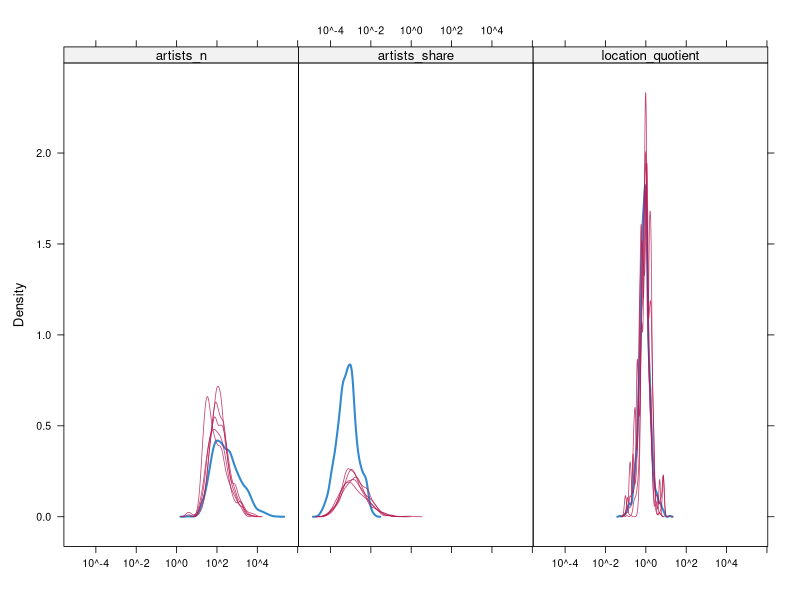
\includegraphics[width=.9\linewidth]{media/diag_dens.png}
\end{center}
\begin{latex}
\pagebreak
\end{latex}
\subsection{Utils}
\label{sec:orgc1e1348}
Group up states into regions: Northeast, South, North Central, West
\begin{minted}[]{r}
assignRegion <- function(state) {
  lvls <- levels(datasets::state.region)

  res <- ifelse(state == "District of Columbia" || state == "Puerto Rico",
	 datasets::state.region[1],
	 datasets::state.region[match(state, datasets::state.name)]
	 )
  return(factor(lvls[res], levels = lvls))
}

df <- artists_mi %>% mutate(region = Vectorize(assignRegion)(state))
\end{minted}

Function to estimate the mode(s) of a univariate distribution, particularly multimodal.
\begin{minted}[]{r}
## from package of the same name
ModEstM <- function(x, ...){
  Density = stats::density(x, ...)
  ###
  data.frame(abciss = Density$x,
	     density = Density$y) |>
    dplyr::mutate(decreasing = c(FALSE, diff(.data$density) < 0),
		  localextremum = c(FALSE, diff(.data$decreasing) != 0),
		  nblocalextrema = cumsum(.data$localextremum)) |>
    dplyr::filter(.data$decreasing) |>
    dplyr::group_by(.data$nblocalextrema) |>
    dplyr::slice(1) |>
    dplyr::arrange(desc(density)) |>
    dplyr::pull(.data$abciss) |>
    list()
}
\end{minted}

\begin{latex}
\pagebreak
\end{latex}
\section{Explore}
\label{sec:orga39b450}
This is a fairly small dataset. Variables of interest are \texttt{artists\_share}, the percentage of workers that are artists, and \texttt{location\_quotient}, the ratio between a certain state's number of workers and the overall US's. \texttt{location\_quotient} can be roughly though of as where an occupation gravitates to. We are also interested in the distribution of values across the US.

To start, Designers are the most popular artist by a long shot, in terms of absolute numbers:
\begin{minted}[]{r}
df %>% group_by(type) %>% summarize(sum(artists_n)) %>% arrange(desc(`sum(artists_n)`))
\end{minted}

\begin{verbatim}
# A tibble: 13 × 2
   type                                       `sum(artists_n)`
   <chr>                                                 <dbl>
 1 Designers                                            935090
 2 Writers And Authors                                  252870
 3 Fine Artists, Art Directors, And Animators           235915
 4 Photographers                                        191120
 5 Architects                                           185495
 6 Producers And Directors                              179995
 7 Musicians                                            170949
 8 Announcers                                            81850
 9 Actors                                                68255
10 Entertainers                                          62115
11 Music Directors And Composers                         59320
12 Landscape Architects                                  42579
13 Dancers And Choreographers                            30220
\end{verbatim}


We can see that there is not much difference in \texttt{artists\_share} across both \texttt{race} and \texttt{region}, note the square root x scale.

\begin{minted}[]{r}
df %>%
  ggplot(aes(x = artists_share, color = race)) +
  geom_boxplot() +
  scale_x_sqrt(breaks = c(1/1000, 1/500, 1/250, 1/125, 1/62.5),
	       labels = scales::label_percent(0.01)) + facet_wrap(vars(region)) +
  theme(axis.text.x = element_text(angle = 90, vjust = 0.5, hjust=1))
\end{minted}

\begin{center}
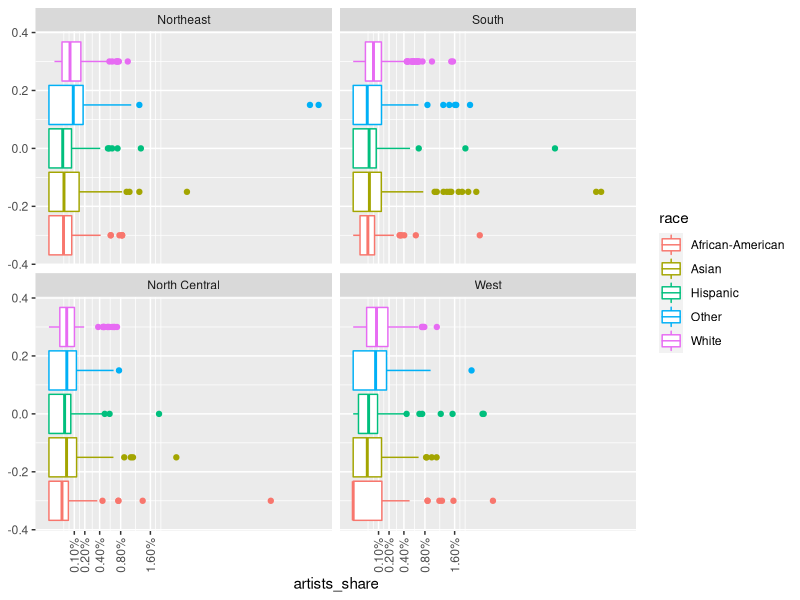
\includegraphics[width=.9\linewidth]{media/race_region_boxplot.png}
\end{center}

We can also inspect how the occupation types differ in relative popularity, the \texttt{artists\_share}. The plots are split by rough order, for clarity. Here, we can see just how much many more Designers there are, even compared to the next closest group, Fine Artists, Art Directors, and Animators.

\begin{minted}[]{r}
modes <- df %>%
  select(type, artists_share) %>%
  group_by(type) %>%
  summarize(mode = ModEstM(artists_share) %>% first %>% first) %>%
  mutate(mode_lvls = cut_number(mode, 4, labels = c("Low", "Med-Low", "Med-High", "High")))

df %>%
    left_join(modes, by="type") %>%
    ggplot(aes(x = artists_share)) +
    geom_density(aes(color = type)) +
    scale_x_continuous(trans = "sqrt", limits = c(0,.015),
		       breaks = c(1/10000, 1/2000, 1/1000, 1/500, 1/250, 1/125, 1/62.5),
		       labels = scales::label_percent(0.01)) + facet_wrap(vars(mode_lvls), ncol = 1) +
    theme(legend.text = element_text(size=6), legend.key.size = unit(4, 'mm'))
\end{minted}

\begin{center}
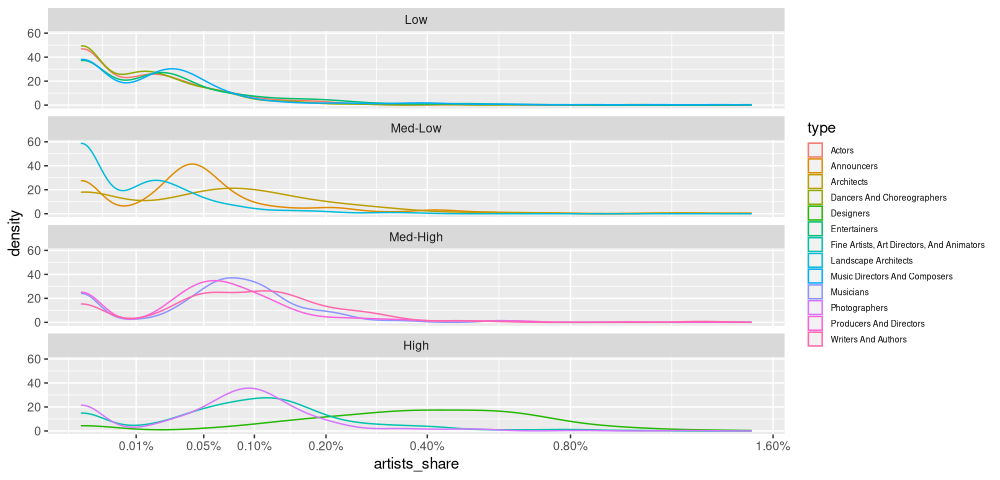
\includegraphics[width=.9\linewidth]{media/share_dens.png}
\end{center}

\begin{latex}
\pagebreak
\end{latex}
\section{GIS}
\label{sec:org66247af}
Create a dataframe with states as rows, for use later in GIS.

\begin{minted}[]{r}
df_state <- df %>% group_by(state) %>%
  summarize(share = mean(artists_share),
	    quot = mean(location_quotient),
	    work = sum(all_workers_n),
	    arts = sum(artists_n))

df_state %>%
  arrange(desc(quot))
\end{minted}

\begin{verbatim}
# A tibble: 52 × 5
   state                   share  quot      work   arts
   <chr>                   <dbl> <dbl>     <dbl>  <dbl>
 1 District of Columbia 0.00366   2.06   5302765  14195
 2 California           0.00173   1.83 258980085 445095
 3 Nevada               0.00128   1.72  19596005  25440
 4 New York             0.00170   1.72 130899860 243345
 5 Hawaii               0.00153   1.32   9776845  13970
 6 Maryland             0.00108   1.17  42499990  48030
 7 Oregon               0.00211   1.15  27256970  42350
 8 Georgia              0.00110   1.14  67268955  67940
 9 Colorado             0.00104   1.12  39905255  51410
10 Florida              0.000922  1.11 131508390 139505
# … with 42 more rows
\end{verbatim}

Import map data and combine with original data.
\begin{minted}[]{r}
library(rnaturalearthhires)

usa <- rnaturalearth::ne_states("United States of America",returnclass = "sf")
usa_df <- right_join(usa, df_state,
		     by = c("name" = "state")) %>%
  rename(`Location Quotient` = quot,
	 `# All Workers` = work,
	 `# Artists` = arts,
	 `Artist Proportion` = share)
\end{minted}

Map out the four relevant variables:

\begin{minted}[]{r}
## whole us:  xlim = c(-180, -65)

## make function over fill and palette
## fill = c(share, quot, work, arts)
constructMap <- function(fill = quot){
  palette <- switch(fill,
		  "Location Quotient" = scale_fill_gradient2(high = "#b2182b", # colorbrewer RdGy
							     mid = "#ffffff",
							     low = "#00ffff", midpoint = 1),
		  "# All Workers" = scale_fill_distiller(palette = "Reds", direction = 1,
						label = scales::label_number(suffix = "M", scale = 1e-6)),
		  "# Artists" = scale_fill_distiller(palette = "Blues", direction = 1,
						label = scales::label_number(suffix = "K", scale = 1e-3)),
		  "Artist Proportion" = scale_fill_distiller(palette = "Purples", direction = 1,
						 labels = scales::label_percent(0.01)),
		  stop("Not a valid fill value"))

  world <- usa_df %>%
    ggplot(aes(fill = !!sym(fill))) +
    geom_sf() +
    palette

  mainland <- world + coord_sf(xlim = c(-130, -69), ylim = c(23, 49)) +
    ggtitle(fill) + theme(plot.title = element_text(size = 20, hjust = 0.5), legend.title=element_blank())
  alaska <- world + coord_sf(xlim = c(-180, -130), ylim = c(51, 71), datum = NA) + theme(legend.position="none")
  hawaii <- world + coord_sf(xlim = c(-161, -154), ylim = c(18, 23), datum = NA) + theme(legend.position="none")

  mainland +
    annotation_custom(
      grob = ggplotGrob(alaska),
      xmin = -140, xmax = -110,
      ymin = 23, ymax = 32) +
    annotation_custom(
      grob = ggplotGrob(hawaii),
      xmin = -124, xmax = -100,
      ymin = 23, ymax = 28)
}

gridExtra::grid.arrange(constructMap("# All Workers"), constructMap("# Artists"),
			constructMap("Location Quotient"), constructMap("Artist Proportion"))
\end{minted}

\begin{center}
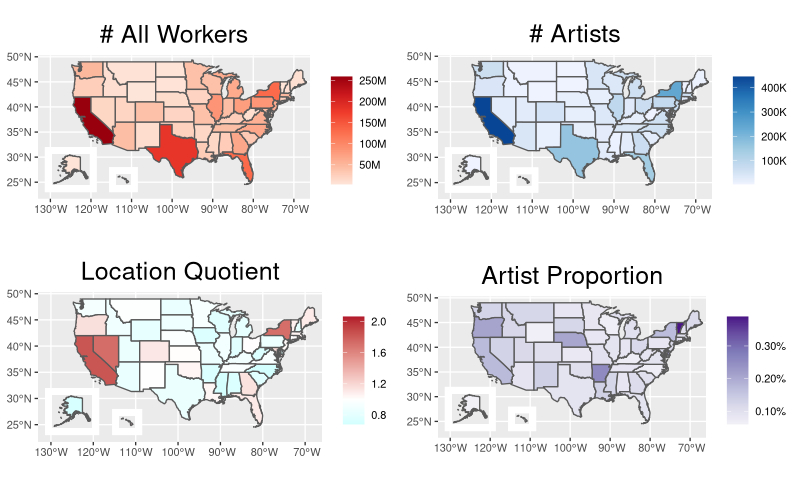
\includegraphics[width=.9\linewidth]{media/gis_vars.png}
\end{center}

We can see that both the total number of workers and total number of artists distribute similarly, primarily in California, Texas, New York, and Florida. Likewise, this means the proportion of artists is fairly uniform across the country. The location quotient tells us that artists in general concentrate in California, Nevada, and New York.

To inspect this quotient relationship, plot by each artist type:

\begin{minted}[]{r}
df %>%
  group_by(state, type) %>%
  summarize(Quotient = mean(location_quotient)) %>%
  rename(job = type) %>%
  right_join(usa, by = c("state" = "name")) %>%
  ggplot(aes(fill = Quotient)) +
  geom_sf(aes(geometry = geometry)) +
  facet_wrap(vars(job), ncol = 3) +
  scale_fill_gradient2(high = "#b2182b", # colorbrewer RdGy
		       mid = "#ffffff",
		       low = "#00ffff", midpoint = 1) +
  coord_sf(xlim = c(-130, -69), ylim = c(23, 49)) +
  theme(legend.position = c(0.65, 0.08),
	legend.direction = "horizontal",
	legend.background = element_rect(fill = "gray90", colour = "black"))
\end{minted}

\begin{center}
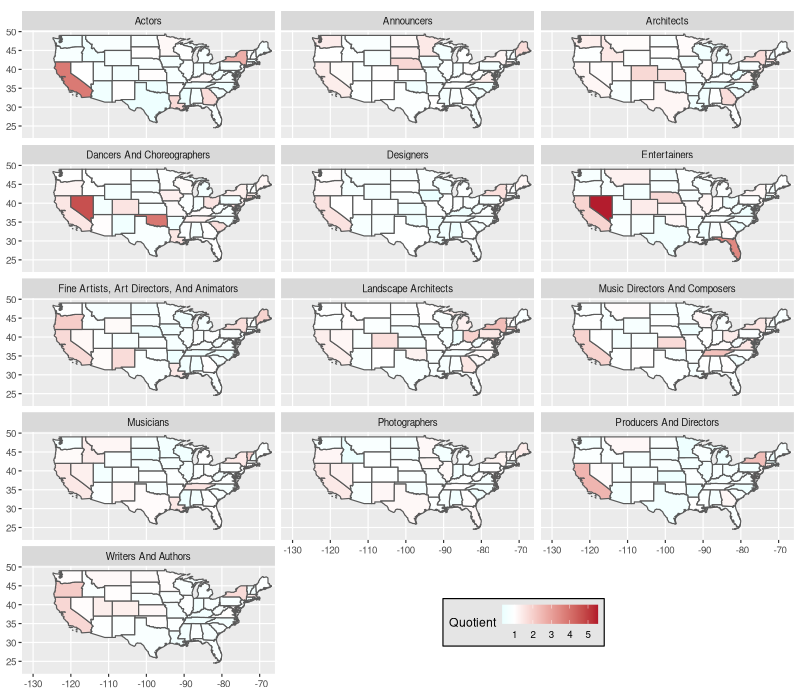
\includegraphics[width=.9\linewidth]{media/gis_quot.png}
\end{center}

Some interesting points:
\begin{itemize}
\item Actors \& Producers And Directors congregate in California, New York, and Georgia
\item Nevada is where Dancers and Choreographers \& Entertainers are
\item The scale is highly skewed by Actors, Dancers And Choreographers, \& Entertainers, which I attribute to Hollywood and Las Vegas.
\end{itemize}

\begin{latex}
\pagebreak
\end{latex}
\section{Resources}
\label{sec:org2b46d5c}
\begin{itemize}
\item MICE: \url{https://www.gerkovink.com/miceVignettes/Convergence\_pooling/Convergence\_and\_pooling.html}
\item \url{https://r-spatial.org/r/2018/10/25/ggplot2-sf-3.html}
\end{itemize}
\end{document}